\documentclass{pgnotes}

\title{Power distribution}

\begin{document}

\maketitle

\section{Distribution path}

\autoref{fig:power-distribution} shows the basic power distribution hierarchy in a data centre.

\begin{figure}[htbp]
  \centering
  \includegraphics[width=0.5\linewidth]{power_distribution_diagram}
  \caption{Power distribution schematic}
  \label{fig:power-distribution}
\end{figure}

We will consider the distribution path looking \textit{backwards} from the IT equipment towards the incoming mains.


\subsection{Power distribution unit (PDU)}

Each rack normally has a power distribution unit, which is no more complicated than a multiplug adapter:
\begin{itemize}
\item PDU can be mounted vertically in the back of rack or in a rack space (facing in or out).
\item PDUs are available with various combinations of input and output connectors.
\item PDUs may or may not have surge protection and switches.
\item Maximum current will usually be dependent on the connector type on the input to the PDU.
\item ``Smart'' PDUs are available that can measure power demand and turn on/off sockets remotely. (See later on!)
\end{itemize}

\newpage
\subsection{Common connectors}

\autoref{tab:common-mains-plugs-sockets} shows the most common mains power connectors (plugs and sockets) that will be encountered in a data centre environment.

\begin{table}[htbp]
  \centering  
  \begin{tabular}{l r r r}
    \toprule
    \textbf{Type} & $I_{\mbox{max}}$ & \textbf{Male} & \textbf{Female} \\
    \midrule
    BS~1363 & \SI{13}{\ampere} & ~ & ~ \\
    \midrule
    IEC~C13/14 & \SI{10}{\ampere} & C14 & C13 \\
    \midrule  
    IEC~C19/20 & \SI{16}{\ampere} & C20 & C19 \\
    \midrule  
    IEC~60309 & \SI{16}{\ampere} & ~ & ~ \\
    \bottomrule
  \end{tabular}
  \caption{Common connector types}
  \label{tab:common-mains-plugs-sockets}
\end{table}

Of particular interest are the C13/15/19 connectors, \autoref{fig:c13-15-19-connectors}

\begin{figure}[htbp]
  \centering
  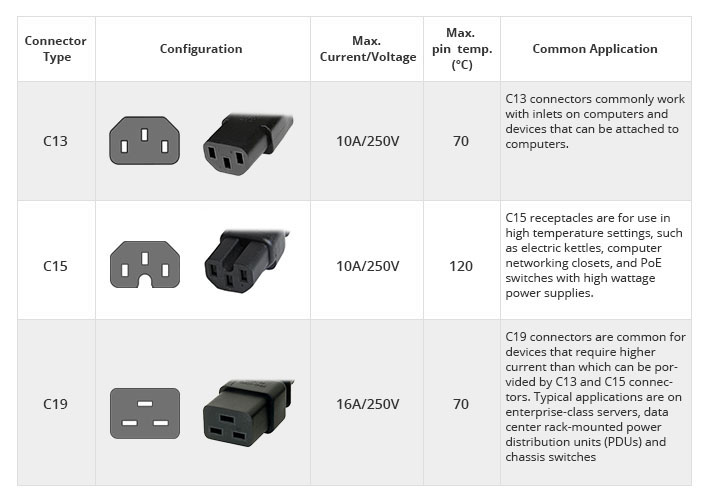
\includegraphics[width=0.9\linewidth]{connectors}
  \caption{C13/15/19 connectors}
  \label{fig:c13-15-19-connectors}
\end{figure}

\section{Disturbances}

Our IT equipment expects clean power with its key parameters (voltage, frequency) maintained within allowable tolerences (\SI{230}{\volt} RMS, \SI{50}{\hertz}).
Waveform must be a \textit{clean} sine wave, not \textit{distorted}.

\subsection{Disturbance types}

\begin{description}
\item[Blackout:] total loss of power.
\item[Surge/sag:] \textbf{short-term} (0.5 of a cycle up to 1 minute) voltage variations:
\begin{description}
\item[Surge or spike] is a short-term high-voltage condition more than \SI{110}{\percent} of the nominal value.
\item[Sag] is a short-term low-voltage condition.
\end{description}

\item[Over and under-voltage] conditions that \textbf{persist for time periods} ranging from minutes to days:
\begin{description}
\item[Over-voltage] is increased mains voltage.
\item[Under-voltage] is reduced mains voltage.  (Formerly: brownout)
\end{description}

\item[Frequency fluctuations] away from \SI{50}{\hertz} for long and short periods.

\item[Waveform distortion] when the mains voltage waveform no longer is a sinusoid.
This can manifest in a number of ways: offsets, harmonics, notching and noise.

\end{description}
\newpage

\begin{figure}[htbp]
  \centering
  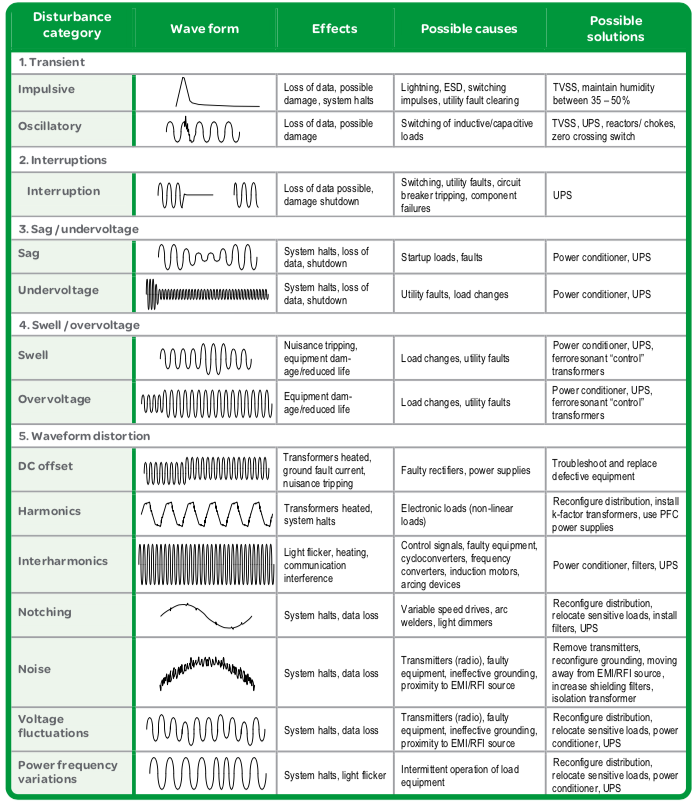
\includegraphics[width=0.9\linewidth]{disturbances}
  \caption{Disturbances}
  \label{fig:disturbances}
\end{figure}

\clearpage
\newpage

\subsection{CBEMA curve}

Undesirable conditions are generally less disruptive the shorter that they persist for.
This includes disturbances in the power supply.
The Computer Business Equipment Manufacturers Association (CBEMA) in the 1970s generated a curve that partitioned voltage events and times into acceptable and unacceptable region.
The Information Technology Industry Council (ITIC) adapted the curve in the 1990s, which was most recently updated in 2000, \autoref{fig:itic-cbema-curve}

\begin{figure}[htbp]
  \centering
  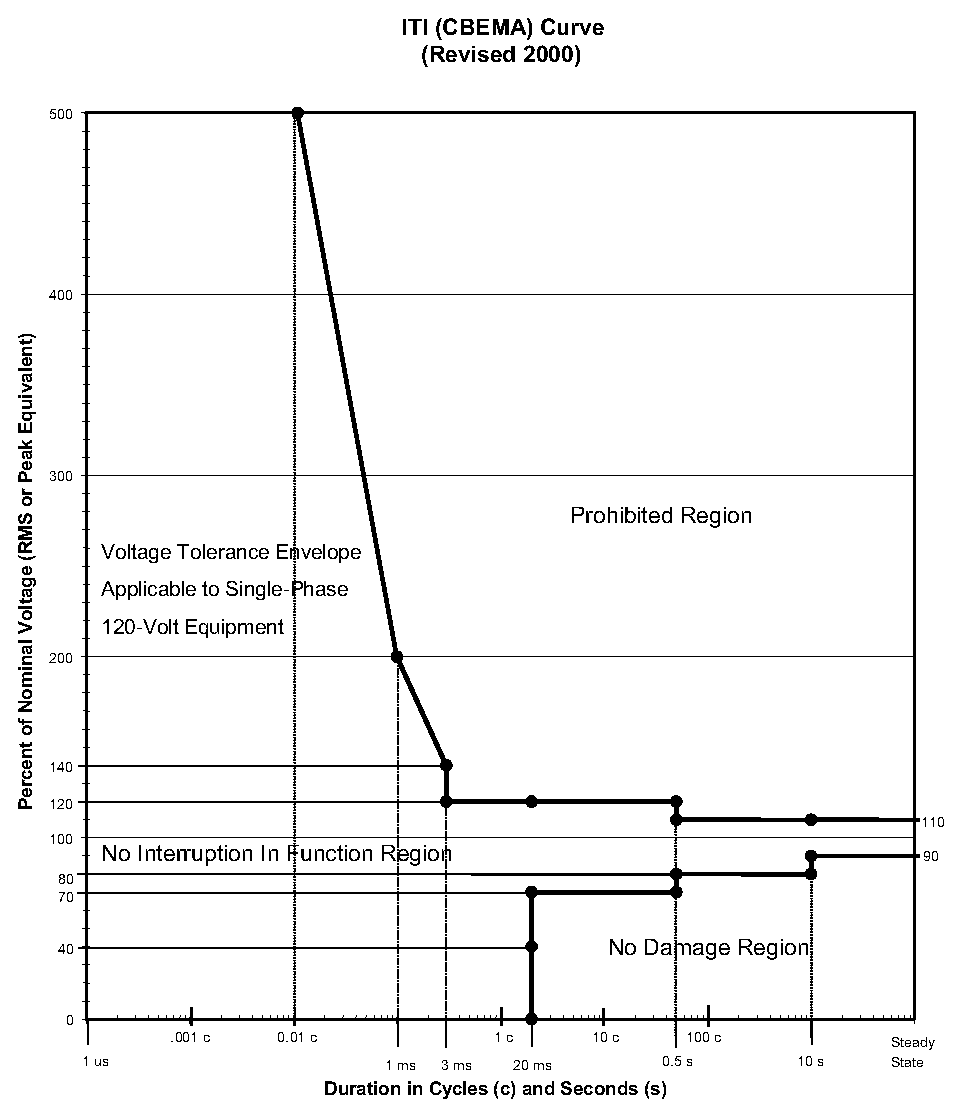
\includegraphics[width=0.7\linewidth]{iti_cbema_curve}
  \caption{ITI CBEMA Curve 2000}
  \label{fig:itic-cbema-curve}
\end{figure}

\newpage

\section{Uninterruptible Power Supplies (UPS)}

\subsection{Key Components}
UPS units are complex devices but contain a number of key building blocks you should know: 
\begin{description}
\item[Battery] as an energy storage medium.
  Common types include: Lead-Acid, Nickel-Cadmium (NiCd), Nickel Metal Hydride (NiMH), Lithium-Ion. 
\item[Rectifier] to convert mains AC to DC for battery charging.
\item[Inverter] to take DC and convert it to AC at a given voltage and frequency.
\item[Transfer switch] to swap between two sources of power. Can be a mechanical relay or contactor\footnote{A contactor is the conventional name used for a large relay able to switch many amperes of current.} but is more usually solid-state, called a \textit{static transfer switch} or STS.
\item[Surge suppressor:] a solid-state device that reduces voltage by letting current flow to earth when a voltage exceeds the so-called \textit{let through} voltage.
\end{description}


\subsection{Form factors}

UPS units are available in various form factors:
\begin{description}
\item[Freestanding / tower] similar to PC powering a single device or multiple devices via a PDU.  Usually located adjacent to the IT equipment.
\item[Rackmount] powering a single device or multiple devices via a PDU. Usually co-located inside the same rack as the IT equipment.
\item[Floor-standing] UPS devices located within the IT environment itself or in another part of the facility. These normally supply multiple IT loads and are often managed by facilities rather than IT personnel. 
\end{description}


\newpage
\subsection{UPS types}

There are three main categories of UPS: standby, line-interactive and double conversion. 
%For a thorough treatment of the different types of UPS systems see \citet{rasmussen:2011:the-different}.
All UPS devices will protect against blackout (for as long as their batteries last).

\subsubsection{Standby}

A standby UPS normally just passes the utility through to the output, while performing basic surge suppression, \autoref{fig:standby-ups-schematic}.

\autoimage{ups_standby_schematic}{Standby UPS schematic (APC)}{standby-ups-schematic}

The battery is charged from the mains.
Under failure of the mains supply, the UPS will use its inverter to generate AC.
The transfer switch changes the output from utility to inverter.

The standby UPS protects against blackouts and small surges/sags whilst remaining online.
It will transfer to inverter supply in the case of under/over voltage conditions.

\subsubsection{Line interactive}

A line interactive UPS is capable of correcting reasonably small under/over voltage conditions \textbf{whilst remaining online}, \autoref{fig:line-interactive-ups-schematic}.

\autoimage{ups_line_interactive_schematic}{Line interactive UPS schematic (APC)}{line-interactive-ups-schematic}

The line interactive UPS will correct surges/sags and under/over voltage whilst remaining online.
It will use transfer to battery power to correct issues with AC frequency and waveform quality.

\subsubsection{Double conversion}

The double-conversion UPS differs from the standby and line-interactive UPS in that it doesn't differentiate between online/offline modes of operation.
Double conversion UPS units correct both voltage and frequency disturbances.
\autoref{fig:double-conversion-ups-schematic}.

\autoimage{ups_double_conversion_schematic}{Double conversion UPS schematic (APC)}{double-conversion-ups-schematic}

They consist of a battery bank charged by the mains, from which an inverter generates a clean AC waveform at the right voltage and frequency,


\section{UPS sizing}

UPS sizing needs to consider how much power the UPS is expected to supply (determines inverter size), and for how long (determines battery size).
The reactive / apparent power requirements need to be considered. 

Specifying a UPS is a somewhat inexact process.
A undersized unit will not work, but an oversized unit will.
Therefore, we normally pad calculated requirements by a \SI{20}{\percent} buffer.

\subsection{Real power requirements}

The UPS power required, with padding, can be calculated:
\begin{align}
  P_{\mbox{total}} & = \left ( \sum_{\mbox{devices}} P_{\mbox{device}} \right ) \times 1.2
\end{align}


\subsection{Apparent power}

When sizing power distribution components, we need to consider the so-called Volt-Amp rather than the Watt.
So far we know that the watt is the unit of power.
From the power relation we first met in \autoref{eq:power-P}, $P = V \cdot I$, we might reasonably expect that $\SI{1}{\watt}=\SI{1}{\volt\ampere}$.
However, in real life this isn't the case.

\subsubsection{Reactive power}

In simple loads like incandescent lights and heaters, regardless of size, the current and voltage will be perfectly in phase.
However, with many real-world loads the current wave will lead or more usually lag the voltage wave, becuase of the dynamical nature of the circuits.
\begin{description}
\item[Inductive] loads will cause the current wave to \textit{lag} the voltage wave.
\item[Capacitive] loads will cause the current wave to \textit{lead} the voltage wave.
\end{description}
These loads are the electrical equivalents of a hose or balloon filled with pressurised water, or a large heavy flywheel.

\autoimage{power_factor_07}{Reactive load showing current lagging voltage (Wikipedia)}{power-factor-07}

Let $P$ be the real power, and $Q$ be the reactive power.
The imaginary unit $j$ is such that $j^2=-1 \Rightarrow j=\sqrt{-1}$.
(Some textbooks, including leaving cert maths use $i$ as the imaginary unit, but it is prone to confusion with $i$ meaning current.)
We define the apparent power $S$ by:
\begin{align}
  S & = P + j Q
\end{align}
This is a complex number, which we can think of as the so-called power triangle.
\autoimage{power_triangle}{Power triangle (Wikipedia)}{power-triangle}

The apparent power for sizing purposes of a UPS is then simply the magnitude, $ \left \lvert S \right \rvert $.
\begin{align}
  \left \lvert S \right \rvert ^2 & = P^2 + Q^2 \\
  \left \lvert S \right \rvert & = \sqrt{P^2+Q^2}   
\end{align}

We can also re-arrange this to give the real, $P$, and reactive, $Q$, power components: 
\begin{align}
  \left \lvert P \right \rvert ^2 & = \sqrt{ \left \lvert S^2 \right \rvert - Q^2 } \\
  \left \lvert Q \right \rvert ^2 & = \sqrt{ \left \lvert S^2 \right \rvert - P^2 } \\
\end{align}

\subsubsection{Power factor}
\label{sec:power-factor}

Looking back at the power triangle, \autoref{fig:power-triangle}, the angle $\theta$ encodes the relative breakdown between real and reactive power.
Assuming we know $P$ and $Q$, the angle $\theta$ is simply:
\begin{align}
  \theta = \tan^{-1} \frac{Q}{P} 
\end{align}
We normally consider not the angle $\theta$, but the cosine of it, $\cos \theta$.
This gives us the ratio of real power to apparent power, and it is called the \textbf{power factor}, $PF$: 
\begin{align}
  PF & = \frac{P}{\left \lvert S \right \rvert}
\end{align}
In terms of its interpretation:
\begin{itemize}
\item Power factor is a dimensionless number between $-1$ and $1$.
\item Negative power factors imply a device generating real power, not consuming it. We will assume the power factor here is between $0$ and $1$.
\item Power factor does not tell if current is leading/lagging the voltage. Assumed lagging unless specified.
\end{itemize}

\subsubsection{Apparent power for a single device}

If you have the voltage and amps \textbf{directly} specified for a particular piece of equipment, you can just multiply to get $S$:
\begin{align}
  \left \vert S_{\mbox{device}} \right \rvert & = V \times I 
\end{align}


\begin{example}{VA calculation from voltage and current}{va-calculation-from-voltage-and-current}
  A server's power supply has a rating plate claiming that it consumes up to \SI{3.5}{\ampere} when connected to a \SI{230}{\volt} supply.
  Determine the VA.
  \tcblower
  Here, we simply use the $V$ and $I$ ratings as given.
  \begin{align}
    \left \lvert S \right \rvert & = V \times I \\
                                 & = 230 \times 3.5 \\
                                 & = \SI{805}{\volt\ampere}
  \end{align}
\end{example}


If you have the power drawn by the device in watts, and you know the power factor, determine $\left \lvert S \right \rvert$ by calculating:
\begin{align}
   \left \lvert S_{\mbox{device}} \right \rvert & = \frac{P}{PF }
\end{align}
If you're not given a power factor, $PF = 0.8$ will usually work, but state that assumption.

\begin{example}{VA calculation from power}{va-calculation-from-power}
  The specification sheet for a server shows that it consumes up to \SI{250}{\watt}.
  Determine the VA requirement.
  \tcblower
  Given the information we have, we will assume a power factor of 0.8.
  \begin{align}
    \left \lvert S \right \rvert & = \frac{P}{PF} \\
                                 & = \frac{250}{0.8} \\
                                 & = \SI{312.5}{\volt\ampere}
  \end{align}
\end{example}


\subsubsection{Apparent power for multiple devices}

Sum up the VA requirements, remembering to apply the power factor (if not uniform) to each device before summation.
The padding is normally added post summation. 
\begin{align}
  \left \lvert S \right \rvert _{\mbox{total}} & = \left ( \sum_{\mbox{devices}} \left \lvert S_{\mbox{device}} \right \rvert \right ) \times 1.2
\end{align}

\subsection{Runtime}

Runtime for a UPS is normally determined using the sizing chart on the specification sheet.

Runtime can often be extended by adding additional battery packs.

\subsubsection{Battery capacity}

The capacity is specified in units of \si{\ampere\hour}.
This means that the battery can supply the given number of amperes of current for one hour.
\begin{align}
  \mbox{hours available} & = \frac{\mbox{capacity}}{\mbox{current}}
\end{align}
Alternatively it can trade off the amount of current delivered against the time period.





\begin{example}{Battery capacity calculation}{battery-capacity-calculation}
  A \SI{12}{\volt} battery has a capacity of \SI{80}{\ampere\hour}.
  It is to supply a load that requires a constant \SI{5}{\ampere}.
  Calculate how many hours would this battery last assuming it was 100\% charged when connected to the load.
  \tcblower
  \begin{align}
    \mbox{hours available} & = \frac{80}{5} \\
                           & = \SI{16}{\hour} 
  \end{align}
\end{example}

\end{document}


